\label{fnt6.1.2-4}

\begin{wrapfigure}{R}{0.5\textwidth}
	\vspace{-35pt}
	\begin{center}
	\begin{tikzpicture}[thick,scale=0.65, every node/.style={transform shape},background rectangle/.style={fill=white}, show background rectangle]
		% draw a 10x7.5 grid in light gray with 5mm grid spacing
		\draw[step=.5cm,gray,very thin] (0,0) grid (10,7.5);
		% draw a darker grid in light gray with 2.5mm grid spacing
		\draw[step=2.5cm,gray,thick] (0,0) grid (10,7.5);
    
		% draw the first arrow; "Stealth" is the name of the arrowhead, and it's capitalized, so that it's scalable
		\draw[-{Stealth[scale=1.2]}, line width=1.5pt] (6,5.5) -- (2,5.5);
    
		% draw the vector equation on top of the first vector
		\draw (4,5.5) node[above=6pt,align=center] {$\Sigma \vec{F} = \vec{F_1} + \vec{F_2} + \vec{F_3}$};
    
		% draw object node
		\draw (5,1) node[circle,minimum size=6pt,fill,inner sep=1pt]{} node[below=3pt]{object};
    
		% draw the second arrow, with descriptor F1
		\draw[-{Stealth[scale=1.2]}, line width=1.5pt] (5,1) -- (3,2) node[above=3pt]{$\vec{F_1}_\text{ on object}$};
    
		% draw the second arrow, with descriptor F2
		\draw[-{Stealth[scale=1.2]}, line width=1.5pt] (5,1) -- (9,5) node[above=3pt]{$\vec{F_2}_\text{ on object}$};

	\end{tikzpicture}
	\end{center}
	\vspace{-10pt}
\end{wrapfigure}

%\begin{wrapfigure}{R}{0.5\textwidth}
%	\vspace{-35pt}
 % 	\centering
%	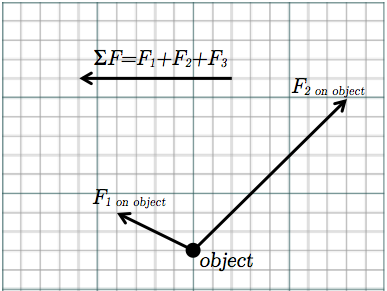
\includegraphics[height=150pt]{fnt612-4-vectors}
%	\vspace{-10pt}
%\end{wrapfigure}

\noindent Vectors $\vec{F}_\text{1 on object}$, $\vec{F}_\text{2 on object}$, and $\vec{F}_\text{3 on object}$ are all exerted on an object, adding together to form a net force vector, $\Sigma \vec{F}$, as shown in the graph to the right. However, only vectors $\vec{F}_\text{1 on object}$, $\vec{F}_\text{2 on object}$, and $\Sigma \vec{F}$ are known.\\

\noindent On a separate piece of graph paper, use the properties of vector addition to graphically determine the vector $\vec{F}_\text{3 on object}$.